%---------------------------------------------------------------------------------
\chapter{Spectral Efficiency Techniques in Aeronautical Communications: A Literature Review}
\label{chap:lit_review}
%---------------------------------------------------------------------------------
\section{Introduction}
To adequately cope with data communications demands, the aviation community have identified several candidate technologies for various flight domains. However, efficiently utilizing the aeronautical spectrum is still an issue, which can be addressed in the context of the following questions.

\begin{itemize}
	\item \textit{Which of the available spectral efficiency techniques can be adopted to improve spectral utilization in an aeronautical context?}
	\item \textit{How can the coexistence of legacy, existing and upcoming aeronautical communication technologies on a common aeronautical spectrum be managed?}
\end{itemize}

To this end, the state-of-the-art in aeronautical communications is first presented in this chapter. Thereafter, studies on aeronautical channel modeling are discussed. In particular, various propagation characteristics, e.g., fading scenarios, are present for different flight domains, which must be properly modeled to provide accurate analysis of any proposed aeronautical communication system (ACS). Suitable spectral efficiency techniques that can be adopted for aeronautical communications that are then presented and discussed from the aeronautical communications perspective.


\section{An Overview of Aeronautical Communications}
% brief history of aeronautical communications
Digital communication systems have long been employed in aeronautical communications for both A/A and A/G communication links. Early ACSs operated in the High Frequency (HF) band, rendering such systems to be susceptible to static and atmospheric noise \cite{stacey2008aeronautical}. Despite the development of Aircraft Communications Addressing and Reporting System (ACARS) and VHF digital link (VDL) from the late 1970's, HF ACSs e.g. HF-ACARS, are still retained \cite{stacey2008aeronautical}. This is because the propagation characteristics of the HF band enabled aircrafts to communicate over long distances in the absence of VHF coverage, particularly for flights over oceans or remote places. 

% motivations for FCI and the identified candidate technologies
Nonetheless, the aviation community has been on the search for newer generations of aeronautical data communication systems to adequately meet data communication demands in the near future. The joint European-American Future Communications Infrastructure (FCI) study, along with NextGen and SESAR as accompanying programs, is one such research initiative \cite{neji2013survey}. Specifically, the FCI study was tasked with recognizing possible communications technologies for future aeronautical communications over three phases. Phase one consists of identifying candidate technologies. Phase two concentrates on further adopting and adapting the selected candidate technologies for aeronautical applications and phase three culminates the FCI study with the implementation of required infrastructure on a global scale. It was noted in \cite{neji2013survey} at the time of publication that phase one had already been concluded, with a range of possible technologies identified. The RF bands used for different flight domains have also been identified. Flight domain in this sense refers to the type of terrain that the aircraft is operating in, e.g., when the aircraft travels on the airport/tarmac surface or fly over continental or remote places e.g. oceans, desert.

For surface communications i.e. airport/tarmac, AeroMACS was chosen \cite{neji2013survey,fistas2009future,ehammer2011aeromacs}. AeroMACS is an OFDM system with adaptive modulation based on the WiMAX standard, with data modulated either via QPSK, 16QAM or 64QAM depending on the link quality, i.e., Received Signal Strength Indicator (RSSI) \cite{budinger2011aeronautical,fistas2009future}. A feedback channel is also used to notify the transmitter of the link quality for the adaptive threshold decision process. When used in the C-band, the short range of AeroMACS signals in the C-band results in a high data rate communications platform with minimum interference. In particular, a performance evaluation of AeroMACS by Ehammer et al. \cite{ehammer2011aeromacs} revealed that for a fixed bit error rate (BER) of $10^{-6}$ and $5\times10^{-5}$, forward link bandwidth utilization of 1379 Kbps and 1738 Kbps were reported respectively. For the reverse link, bandwidth utilization of 684 Kbps and 812 Kbps were reported for a fixed BER of $10^{-6}$ and $5\times10^{-5}$ respectively. Separately, measurements conducted by Bundinger and Hall \cite{budinger2011aeronautical} as a test of the AeroMACS concept revealed an average of 3.89 Mbps to 5.13 Mbps of throughput. Despite noting that the airport surface environment is prone to multipath effects, theoretical channel models were not considered during the measurement tests by the authors.

For flights over remote places, the FCI study decided on satellite communication systems to operate in the L-band \cite{neji2013survey,morlet2011options}. These satellite communication systems are expected to be customized for aeronautical applications due to the inability of conventional or commercial satellite systems to support aeronautical communications \cite{neji2013survey}. One such example of a customized satellite communication system is the Iris program that is currently under development by the European Space Agency \cite{morlet2011options,morlet2010characterisation}. The aim of the Iris program is to enable satellite-based aeronautical communications as a complement to existing terrestrial-based ACSs such as LDACS since the former can cover a wider area than terrestrial-based ACSs \cite{morlet2011options}. Performance evaluation of the Iris program conducted by Morlet et al. \cite{morlet2010characterisation} revealed that for airport/tarmac and continental flight domains, an average throughput of 989 Kbps to 4.4 Mbps can be obtained for the forward link while an average throughput of between 568 Kbps to 728 Kbps can be obtained for the reverse link \cite{morlet2010characterisation}. In \cite{morlet2011options}, computer simulations were conducted for aircrafts operating in different regions (e.g. South and North Atlantic, Europe) and it was found that a maximum forward link throughput of 4.85 Mbps can be obtained. Although the Iris satellite communication system can be used to complement terrestrial ACSs, Morlet et al. \cite{morlet2011options} noted that the Iris satellite communication system can be susceptible to signal reception obstruction, i.e., airframe shadowing, which will be further discussed in the next section, due to aircraft maneuvers. This is on top of potential ground reflection of signals, thus causing multipath propagation effects.

Finally, for continental flights, candidates such as B-AMC and AMACS were noted by Neji et al. \cite{neji2013survey}. In the former, the adaptation of B-AMC for L-band communications was investigated in \cite{rokitansky2007bamc}. In the latter, an L-band All-purpose Multichannel Aviation Communication System (AMACS) based on VDL-4 and cellular GSM technology was considered \cite{eurocontrol2007amacs}, \cite{deneufchatel2007all}. Ultimately LDACS was chosen for continental aeronautical communications although satellite communication systems have not been ruled out completely \cite{neji2013survey}, \cite{fistas2009future}. The selected candidate technology and spectral band for the respective flight domains as part of the FCI study are summarized in Table \ref{table:aeroComms}. Note that the recommendations seen in Table \ref{table:aeroComms} have been agreed upon not only in Europe \cite{budinger2011aeronautical}, \cite{fistas2009future}, \cite{fistas2011future} but also in the United States as well \cite{wichgers2013study}, \cite{budinger2011aeronautical}, \cite{budinger2005technology}. 

%\begin{table}[]
%\centering
%\caption{Spectral bands and candidate technologies identified by the FCI study for various flight phases \cite{neji2013survey}, \cite{fistas2009future}}
%\label{table:aeroComms}
%\begin{tabular}{|p{5cm}|p{5cm}|p{2cm}|}
%\hline
%\textbf{Flight Domain}            & \textbf{Candidate Technology}          & \textbf{Spectral Band} \\ \hline
%Airport/Tarmac                    & AeroMACS                               & C-band                 \\ \hline
%Remote Places e.g. oceans, desert & Satellite Communication Systems        & L-band                 \\ \hline
%Continental                       & LDACS, Satellite Communication Systems & VHF and L-band         \\ \hline
%\end{tabular}
%\end{table}

\begin{table}[]
\centering
\caption{Spectral bands and candidate technologies identified by the FCI study for various flight phases \cite{neji2013survey}, \cite{fistas2009future}.} 
\label{table:aeroComms}\scalebox{0.85}{
\begin{tabular}{ccc}
\hline
\textbf{Flight Domain}            & \textbf{Candidate Technology}          & \textbf{Spectral Band} \\ \hline \hline
Airport/Tarmac                    & AeroMACS                               & C-band                 \\ 
Remote Places, e.g., oceans, desert & Satellite Communication Systems        & L-band                 \\ 
Continental                       & LDACS, Satellite Communication Systems & VHF and L-band         \\ \hline
\end{tabular}}
\end{table}

As a result of the FCI study, continental communications via LDACS has seen gradual increase in research interest. This is because LDACS must be able to handle the tremendous volume of aircrafts communicating on A/G links. In addition, the choice between the two variants of LDACS namely LDACS-1 and LDACS-2, is yet to be made \cite{jain2011analysis}. Although both operate in the L-band at the physical layer, LDACS-1 is based on FDD-OFDM that adaptively switches between QPSK, 16-QAM and 64-QAM modulation on a 498KHz channel \cite{brandes2009physical}. This is on top of adaptive convolutional coding that chooses between 1/2, 2/3 or 3/4 code rate. Thus, LDACS-1 can provide up to 1373Kbps and 1038Kbps in the forward and reverse link respectively \cite{jain2011analysis}, \cite{brandes2009physical}. LDACS-2, based on GSM and AMACS, uses GMSK modulation with TDD for multiuser access \cite{neji2013survey}, \cite{fistas2009future}, \cite{jain2011analysis}, \cite{abdulkarim2013comparison}. Using GMSK, LDACS-2 is able to provide 270Kbps of raw throughput with a bandwidth of 200 KHz \cite{jain2011analysis}. This is lower than that of LDACS-1 which requires close to 500 KHz. In terms of spectral efficiency, Jain et al. \cite{jain2011analysis} noted that LDACS-1 can support up to 2.76 bits/s/Hz and 2.08 bits/s/Hz for forward and reverse links respectively. For LDACS-2, 1.3 bits/s/Hz was reported although this number may be lower when coding and overhead costs are considered \cite{jain2011analysis}.

Invariably, LDACS-1 will be able to provide higher data rate communications at a cost of higher spectral resource requirements. Conversely, LDACS-2 will require less spectral resources albeit at lower data rate communications. Evidently, evaluation studies between LDACS-1 and LDACS-2 are already being carried out \cite{neji2013survey}, with the specifications of LDACS-1 and LDACS-2, appropriate prototype developments, e.g., via simulator frameworks such as in \cite{graupl2015method}, aeronautical channel modeling and most crucially, potential interference from existing L-band legacy systems \cite{neji2013survey}, \cite{jain2011analysis}, \cite{brandes2009physical} \cite{epple2014overview} being taken into consideration. These legacy systems include Distance Measurement Equipment (DME), Tactical Air Navigation (TACAN), Universal Access Transceiver (UAT), Secondary Surveillance Radar (SSR), satellite systems, e.g., Global Positioning System (GPS), and telecommunication standards, such as Global Systems for Mobile (GSM) communications and Universal Mobile Telecommunications System (UMTS) \cite{neji2013survey}, \cite{epple2014overview}. Of these systems, Jain et al. \cite{jain2011analysis} noted strong interference from DMEs and telecommunication equipments. In particular, Jamal and Matolak \cite{jamal2017fbmc} showed that interference from DMEs and telecommunication equipments can be detrimental, especially to wideband systems such as LDACS-1. 

Improvements to the proposed LDACS-1 system have also been studied. For instance, Brandes et al. \cite{brandes2009physical} proposed oversampling and zero-padding (referred to as Pulse Blanking in \cite{brandes2009physical}) to mitigate interference from legacy systems. However, this reduces the overall throughput. Similarly, works such as \cite{bhaindl2013overview} and \cite{mschnell2014current} have proposed to extend LDACS-1 for navigational purposes to replace navigation systems in a bid to reduce congestion on the L-band. The adaptation of LDACS-1 as an Alternative Positioning, Navigation and Timing (APNT) solution was presented by Schnell et al. \cite{schnell2011using}. Based on signal latency, the relative distance between aircraft and ground station can be estimated via symbol synchronization. In addition to distance, an aircraft's position can also be estimated (via Weighted Least Squares or Extended Kalman Filter) once the distance to at least three ground stations has been estimated. Accuracies of up to 100m have been reported by using the proposed navigation methods. 

Apart from manned A/G communications, LDACS has also been considered for UAV CNPC links. For instance, Matolak \cite{matolak2015unmanned} cited LDACS-1 and LDACS-2 as potential candidates for future CNPC systems. In terms of future ACSs for A/A communications, Schnell et al. \cite{schnell2014ldacs} noted that this was beyond the scope of both SESAR and NextGen although ADS-B might be a possible future A/A communications technology. Nonetheless, despite LDACS being the selected candidate technology for continental A/G communication links, issues such as standardization, interference management and spectral resource allocation are crucial challenges \cite{neji2013survey} that must be tackled by the aviation community in due time. A summary of the studies that have conducted performance evaluations on the candidate technologies can be seen in Table \ref{table:sumCandidateTech}.

\begin{table}[]
\centering
\caption{Performance evaluation studies conducted for candidate technologies}
\label{table:sumCandidateTech}
\scalebox{0.9}{
\begin{tabular}{ccc}
\hline
\textbf{Candidate Technology}   			& \textbf{Performance Metric(s)}  			& \textbf{References} 							\\ \hline \hline
AeroMACS                    					& Throughput 									& \cite{budinger2011aeronautical} 	\\ 
AeroMACS                    					& Throughput 									& \cite{ehammer2011aeromacs}  			\\ 
Satellite Communication System (Iris)	& Throughput, Antenna Gain    & \cite{morlet2011options}        	\\ 
Satellite Communication System (Iris)	& Throughput                  & \cite{morlet2010characterisation} \\ 
LDACS	1, LDACS-2	                    & Throughput                  & \cite{jain2011analysis}           \\ 
LDACS	1, LDACS-2	                    & BER, Power Spectral Density & \cite{jamal2017fbmc}        \\ 
LDACS	1	                    					& Latency, Packet Loss Rate   & \cite{graupl2015method}           \\ 
LDACS	1	                    					& BER													& \cite{brandes2009physical}        \\ \hline
\end{tabular}}
\end{table}

\section{Aeronautical Channel Modeling}
The characterization of accurate aeronautical channel models for common A/G and A/A communications scenarios has been extensively studied in the literature. Statistical channel models for A/G communications was studied by Haas \cite{haas2002aeronautical}. The study involved analyzing the channel model of an aircraft communicating with a ground station in en route, arrival/takeoff, taxi and parking scenarios, as seen in Table \ref{table:haasFading}. 

\begin{table}[]
\centering
\caption{Fading environments for the various flight scenarios \cite{haas2002aeronautical}.} 
\label{table:haasFading}\scalebox{0.9}{
\begin{tabular}{ccc}
\hline
\textbf{Flight Scenario}				& \textbf{Fading Environment(s)}	& \textbf{Average Rician $K$ Factor} \\ \hline \hline
En route												& Rician and Rayleigh 						& $15dB$ \\
Arrival/Takeoff 								& Rician and Rayleigh 						& $15dB$ \\
Taxi														& Rician and Rayleigh 						& $6.9dB$ \\
Parking                 				& Rayleigh 												& - \\ \hline
\end{tabular}}
\end{table}

The en route scenario can be characterized by an aircraft communicating with a ground station while at cruising altitude with a speed of 17m/s to 440m/s. The arrival/takeoff scenario can be characterized by A/G communications between an aircraft and ground station during landing or takeoff with a speed of 25m/s to 150 m/s. For both the en route and arrival/takeoff scenarios, Rician and Rayleigh fading are assumed for the line-of-sight (LOS) and non line-of-sight (NLOS) components respectively with an average $K$ factor of 15dB. The taxi scenario occurs when an aircraft is communicating with a ground station while traveling on the airport surface with a speed of 0m/s to 15m/s. In this scenario, Rician and Rayleigh fading are also assumed for the LOS and NLOS components respectively with an average $K$ factor of 6.9dB. Finally, the parking scenario occurs when an aircraft is stationary on the airport surface. In this scenario, Haas \cite{haas2002aeronautical} assumed only NLOS communications between aircraft and ground station thus Rayleigh fading is assumed in the parking scenario.

Apart from Haas \cite{haas2002aeronautical}, other recent works on aeronautical channel models have been noted. The propagation characteristics of C-band and L-band signal in A/G communications over water, hilly terrains and suburban/near-urban areas have been investigated as a series of papers in \cite{matolak2017air_water},\cite{sun2017air_hilly} and \cite{matolak2017air_suburban} respectively. In each of these studies, measurements were taken by conducting A/G communications with a ground station when the aircraft is flying over the respective terrains. 

For A/G communications over water surfaces, Matolak and Sun \cite{matolak2017air_water} reported that the free space path loss model can be used to model signal propagation effects, with path loss exponents between 1.5 to 2.2 observed. However, at distances of 10km and above, signal measurements showed that the curved earth two-ray model fits the data more accurately due to water surface reflections. To this end, it was found that the respective $K$ factor for both the L-band and C-band signals are 12dB and 27 to 30dB. Other than Matolak and Sun \cite{matolak2017air_water}, an earlier study by Meng and Lee \cite{meng2011measurements} also reported that the two-ray model can be accurately used to model C-band signal propagation over water surfaces.

The study in \cite{matolak2017air_water} was extended to hilly terrains by Sun and Matolak \cite{sun2017air_hilly}. It was found that, by taking the direction of the aircraft (heading towards or away from ground station) into consideration, the modified log-distance path loss model was able to fit the measured signal accurately. To this end, path loss exponents between 1.6 to 1.8 was observed. From the analysis of the signal measurements, it was also reported that signal reflections from hilly terrain follow a Rician distribution, with an average $K$ factor of 29.4dB and 12.8dB for C-band and L-band respectively.

For A/G communications on airport surface or over suburban/near-urban areas, observations similar to those in \cite{sun2017air_hilly} was reported by Matolak and Sun \cite{matolak2017air_suburban}. Notably, signal propagation path losses in suburban/near-urban areas followed the modified log-distance path loss model with path loss exponents between 1.5 to 2 was observed. For near-urban area, an average $K$ factor of 27.4dB and 12dB was observed for C-band and L-band respectively. In suburban areas, the average observed $K$ factor values for C-band and L-band are 28.5dB and 14dB was observed for C-band and L-band respectively. For airport surface communications, Wu et al. \cite{wu2011airport} observed that the two-ray or log-distance model can accurate model path loss, with an average path loss exponent of 4 and 5.6 reported for the LOS and NLOS components respectively. 

In addition to the studies conducted in \cite{matolak2017air_water}, \cite{sun2017air_hilly}, \cite{matolak2017air_suburban}, the effect of airframe shadowing on A/G communication channels was also recently investigated by Sun et al \cite{sun2017air_shadowing}. Airframe shadowing occurs when an aircraft's body temporarily obstructs the LOS A/G channel between the aircraft and the ground station due to aircraft maneuvers. Sun et al \cite{sun2017air_shadowing} was able to model airframe shadowing loss as a function of an aircraft's roll angle. Signal measurements revealed that an average path loss of 15.5 dB and 10.8 dB for C-band and L-band signals. In addition, it was also observed that airframe shadowing can significantly reduce the Rician $K$ factor for LOS components, with measurements showing a drop of up to 35dB. Furthermore, Sun et al \cite{sun2017air_shadowing} reported that airframe shadowing losses are independent of the link distance and ground station environment. Airframe shadowing can be mitigated by placing additional antennas on the aircraft to maintain LOS A/G communication \cite{sun2017air_shadowing}. However, future ACSs will need to explore other practical solutions because the option of having additional antenna mounting points may not always be available.

\begin{table}[]
\centering
\caption{A summary of propagation environments over various types of terrain.} 
\label{table:propTerrain}\scalebox{0.8}{
\begin{tabular}{ccc}
\hline
\textbf{Terrain}					& \textbf{Average Rician $K$ Factor} 					& \textbf{Path Loss Exponent} \\ \hline \hline
Water Surfaces						& 12dB (L-band), 27dB-30dB (C-band) 					& 1.5 - 2.2 \\
Hilly 										& 29.4dB (C-band), 12.8dB (L-band) 						& 1.6 - 1.8 \\
Airport or Urban/Suburban & 27.4dB-28.5dB (C-band), 12dB-14dB (L-band) 	& 1.5 - 2 \\ \hline
\end{tabular}}
\end{table}

In this section, discussion on accurate modeling of aeronautical channels have been presented. In particular, combinations of Rician and Rayleigh fading are commonly encountered aeronautical communications. Important parameters, such as Rician $K$ factors and path loss exponents, have been characterized by various studies for different scenarios/terrains, as summarized in Table \ref{table:haasFading} and Table \ref{table:propTerrain}. It should also be pointed out that the signal models for various aeronautical scenarios in the current work are based on the parameters in Table \ref{table:haasFading} and Table \ref{table:propTerrain}.

%%%%%%%%%%%%%%%%%%%%%%%%%%%%%%%%%%%%%%%%%%%%%%%%%%%%%%%%%%%%%%%%%%%%%%%%%%%%%%%%%%%%%%%%%%%%%%%%%%%%%%%%%%%%%%%%%%%%%%%%%%%%%%%%%%%%%%%%%%
\section{Potential Spectral Efficiency Techniques in Aeronautical Communications}

Spectral efficiency improvements have long been a topic of interest in the literature, with many techniques that can be potentially adopted for aeronautical communications. For instance, the CR paradigm can be applied for ACSs in A/G communications scenarios. In A/G communications scenarios, legacy ACSs on board aircrafts can continue to operate in the designated spectrum as primary users while allowing newer generations of communication systems to operate as secondary users in overlay (interweave) mode \cite{jacobcognitive}. Such an arrangement can keep interference to legacy systems in check while accommodating newer generations of ACSs on board aircrafts. 

The cognitive radio paradigm can also be adopted for A/A communications between aircrafts (manned or unmanned) in the form of Device-to-Device (D2D) communications. D2D communications can be used to relay signals between nearby aircrafts and ground stations for interference cancellation. Therefore, the quality of A/A and even A/G communications is improved while potential interference from legacy ACSs is reduced. When combined with proper spectrum access management, i.e., CR-based techniques seen in \cite{min2011capacity}, \cite{chen2012downlink}, \cite{xu2014dynamic}, an A/A D2D communications system can also be used for data communications over oceanic or polar flight routes where A/G communications is not possible via signal relaying between aircrafts.

\begin{figure}[]
\centering
\vspace{-2cm}
\includegraphics [width=0.8\columnwidth]{chap2_fig/chap2_fd_gs_system_model.eps} 
\vspace{-2.2cm}
\caption{Multi-user system model with a FD ground station and (a) HD receivers or (b) FD receivers.}
%\vspace{-0.5cm}
\label{fig:chap2_fd_gs_system_model}
\end{figure}

\begin{figure}[]
\centering
\vspace{-2cm}
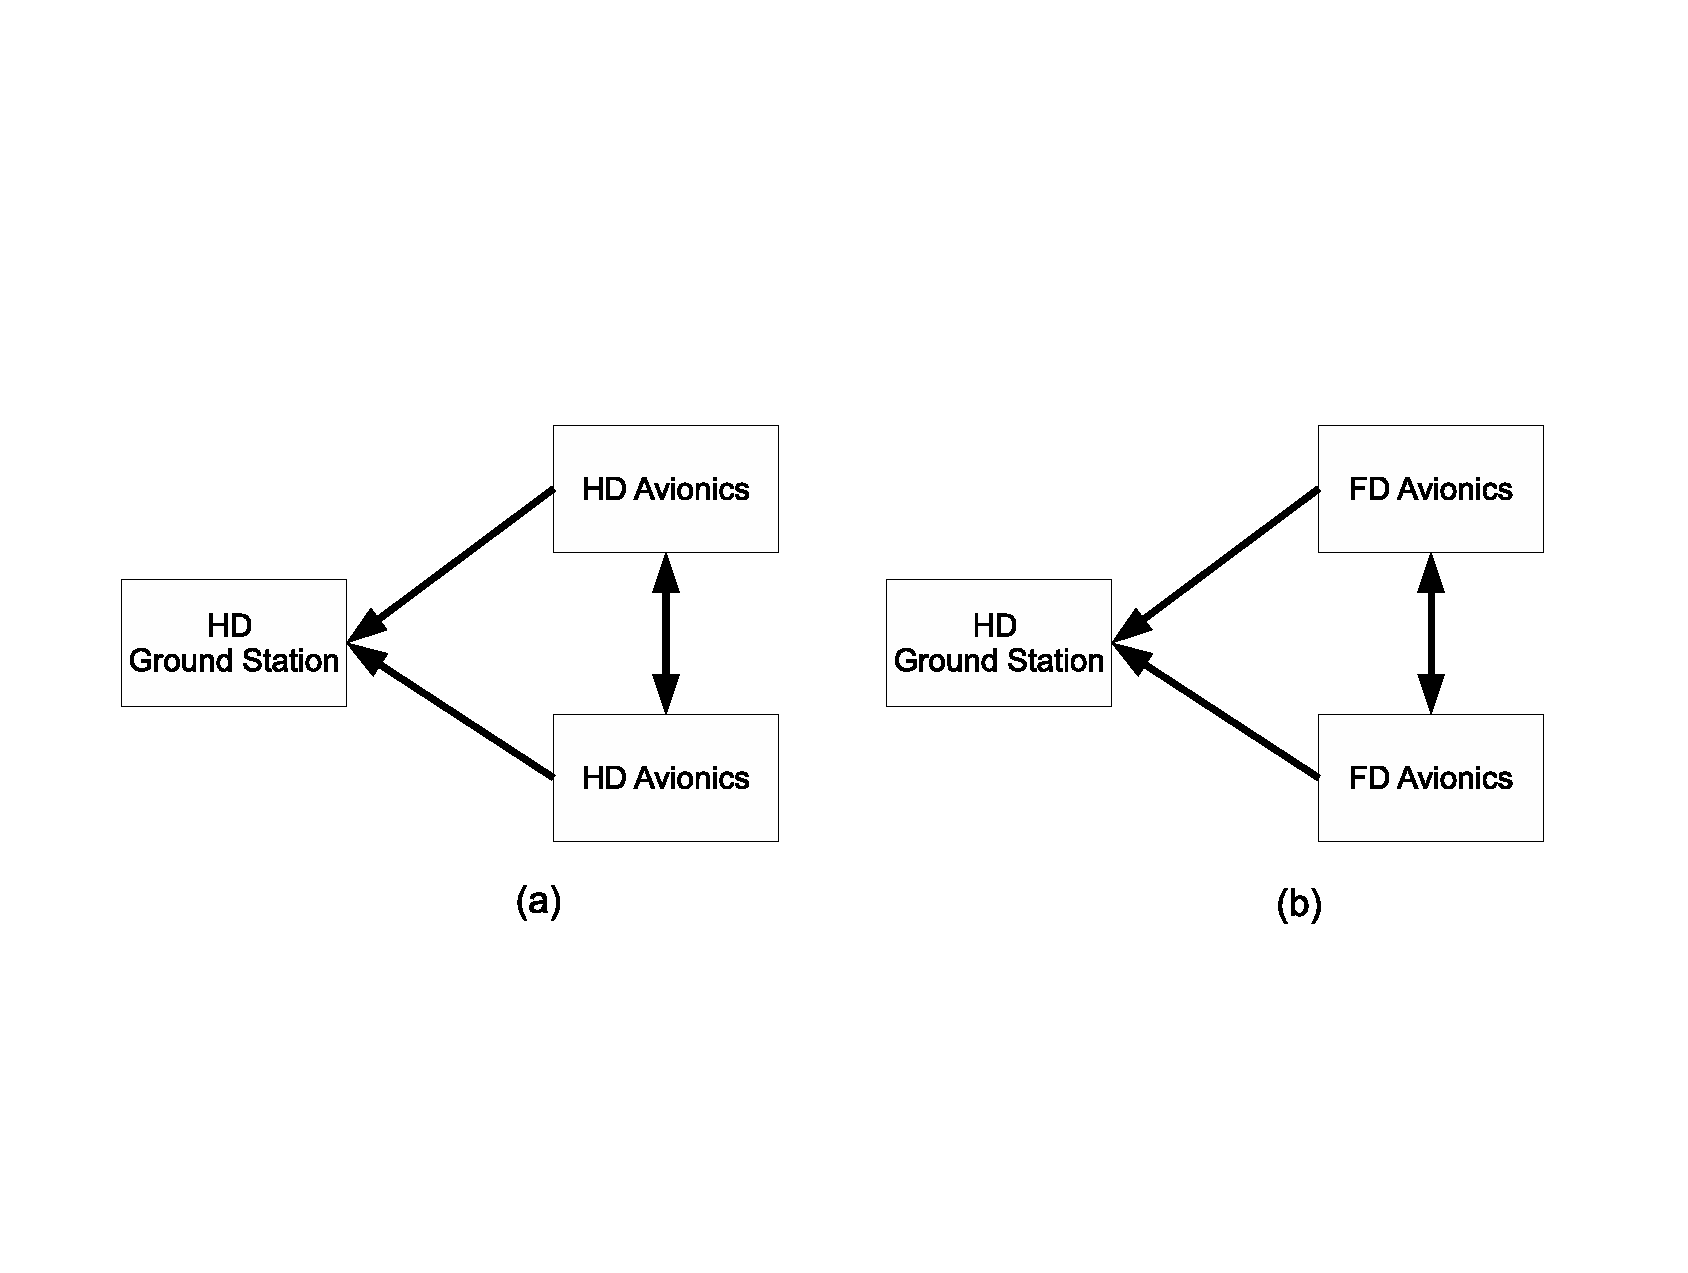
\includegraphics [width=0.8\columnwidth]{chap2_fig/chap2_hd_gs_system_model.eps} 
\vspace{-2cm}
\caption{Multi-user system model with a HD ground station and (a) HD receivers or (b) FD receivers.}
%\vspace{-0.5cm}
\label{fig:chap2_hd_gs_system_model}
\end{figure}

Apart from the techniques discussed earlier, several other spectral efficiency techniques, suitable for aeronautical communications, are available in the literature. However, the current work focuses on improving spectral efficiency in HD and FD-enabled ACSs over A/G links. In HD ACSs, the system model in Fig. \ref{fig:chap2_hd_gs_system_model}a is assumed, where the HD ACS, i.e., avionics, communicates with the ground station (GS). In FD ACSs, as seen in Fig. \ref{fig:chap2_fd_gs_system_model} and Fig. \ref{fig:chap2_hd_gs_system_model}b, self interference (SI) is experienced at the the FD transceivers due to the simultaneous signal transmission and reception. Also, interference at both HD and FD ACSs is also experienced due to the uplink nature of communication. 

Based on the system models seen in Fig. \ref{fig:chap2_fd_gs_system_model} and Fig. \ref{fig:chap2_hd_gs_system_model}, the current work focuses on advanced modulation schemes and In-Band Full-Duplex radio systems to boost spectral efficiency in HD and FD-enabled ACSs, which are practical and efficient spectrum utilization alternatives in aeronautical communications and is discussed in detail in the subsequent subsections.

\subsection{Modulation and Multiplexing Schemes for Aeronautical Communications}
\subsubsection{Modulation Schemes for Aeronautical Communications} 
% Disscuss relevance to aeronautical communications
Current A/G links rely on VDL-2 for data communications. However, the VDL-2 specification employs D8PSK as the modulation of choice to provide for a data rate of 31.5 kbps \cite{stacey2008aeronautical}. Evidently, the achievable data rate of VDL-2 is woefully inadequate if future data communication demands are to be met. To address the low data rate issue of current A/G links, advanced modulation schemes suitable for aeronautical communications can be implemented that either increases the number of bits transmitted per symbol or improves the reliability of communications, i.e., boost the spectral efficiency of ACSs. 

% Discuss techniques that increases the number of bits per transmitted symbol
The hierarchical modulation paradigm has been explored as an alternative to increase the number of bits per transmitted symbol by relying on the quadrant containing the QAM symbol as an additional domain to represent data bits \cite{jiang2005hierarchical,bae2008research} at the cost of signal detection complexity. Modified variants of PSK-based modulation have also been studied to increase the bits carried per symbol. In particular, transmitting additional bits through rotating the QPSK constellation in a specific direction was proposed by Liu et al. \cite{liu1992rotative}. Through the proposed method, an additional bit can be transmitted per QPSK symbol at the cost of higher receiver complexity. More recently, Hong et al. \cite{hong2015additional} proposed rotating the QPSK constellation after the transmission of each block of bits to convey additional bits. Although the detection complexity is not as substantial compared to \cite{liu1992rotative}, the proposed method only achieves a maximum of 16\% boost in throughput.

% Discuss BICM and SSD as techniques that increases reliability
% Present open problems related to aeronautical communications if possible
Apart from increasing transmission rates, enhanced modulation techniques have also been extensively studied to improve reliability. For instance, Bit Interleaved Coded Modulation (BICM) was first proposed by \cite{zehavi19928} to improve the reliability transmissions over Rayliegh fading channels. In particular, the transmitter performs interleaving at the bit level before modulation and vice versa at the receiver \cite{zehavi19928,caire1998bit,li2002bit,zhan2017differential}. BICM has since been extensively studied, with different decoding methods proposed \cite{li2002bit,abotabl2017broadcast} and evaluation over multipath Rayleigh channels conducted \cite{zhan2017differential}. Nonetheless, the increase in reliability for BICM comes at the cost of reduced euclidean distance \cite{li2002bit}.

Signal Space Diversity (SSD), i.e., modulation diversity, is also another technique that has been widely studied to improve communications reliability. SSD was first proposed by Boutros and Viterbo \cite{boutros1998signal} where the in-phase and quadrature phase components of a symbol are rotated and interleaved. The idea is to separately transmit the in-phase and quadrature phase components over a fading channel to diminish the impact of fading \cite{boutros1998signal}. By far, studies pertaining to SSD have looked at code design \cite{mohammed2012modulation} and performance analysis over Nakagami-$m$ \cite{lu2012bit} and Rayleigh \cite{sokun2017spectrally} fading channels. These analysis are useful since Nakagami-$m$ and Rayleigh can be encountered in aeronautical communications. However, suitable code designs for aeronautical communications and the impact of imperfect channel knowledge, particularly for various flight scenarios where Rician fading channels are expected, are open problems that must be addressed.

\subsubsection{Multiplexing Schemes for Aeronautical Communications}

An alternative to meet demands for rising data traffic stemming from aeronautical communications is the non-orthogonal multiple access (NOMA) paradigm. NOMA has been proposed as a next-generation multiple access candidate \cite{dai2015non} in 5G cellular communications. As spectral efficiency is a vital issue that must be addressed in 5G, NOMA, when compared to orthogonal multiple access (OMA) methods, offers spectral efficiency boosts whilst allowing massive connectivity \cite{dai2015non}. Conventional OMA methods such as Frequency Division Multiple Access (FDMA), Time Division Multiple Access (TDMA) and Code Division Multiple Access (CDMA) have traditionally been used to segregate users in terms of channel frequencies (e.g. spectral resources), timeslots or codes. 

However, OMA techniques inherently causes inefficient utilization of spectral resources as users have dedicated resources at the moment of transmitting or receiving signals. NOMA, on the other hand, allows multiple users to simultaneously share the same spectral resources. This is done by allowing an acceptable amount of interference from users simultaneously multiplexed to the same set of spectral resources \cite{dai2015non}. The NOMA paradigm can be well suited for adaptation for aeronautical communications. Interference from nearby aircrafts or ground stations can be canceled while accommodating a large number of aircrafts in the same airspace that are transmitting data via A/G or A/A communication links. To enable resource multiplexing, NOMA techniques can be broadly categorized as Power Domain Multiplexing (PDM) or Code Domain Multiplexing (CDM). 

\begin{figure} []
\centering
\vspace{-0.7in}
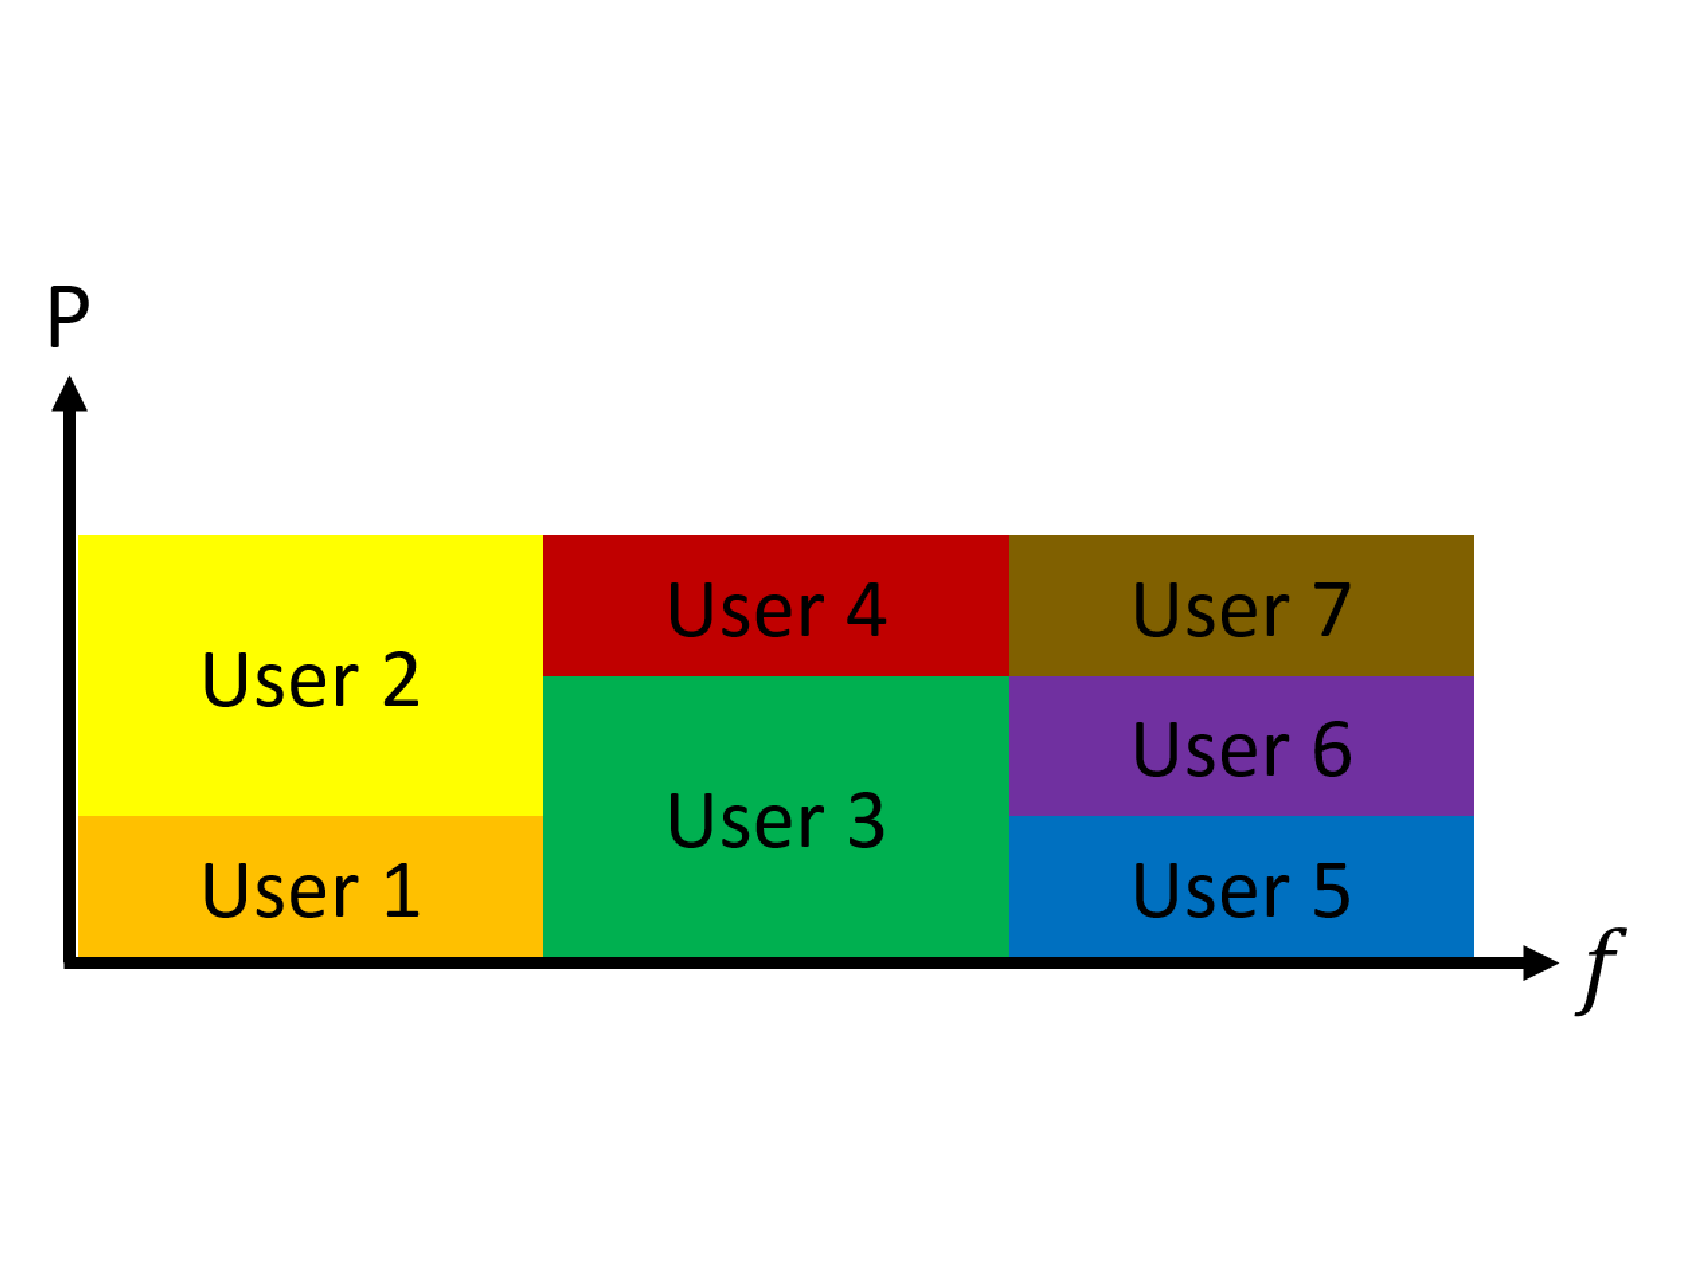
\includegraphics [width=0.6\columnwidth]{chap2_fig/NOMA_fig1.eps}  %ZICRSystemModel.eps} % {LAR.eps}\columnwidth   [width=2\columnwidth] 
\vspace{-0.8in}
\caption{Users in power domain multiplexing are partitioned using transmission power levels.}
\label{fig:6}
\end{figure}

In PDM-NOMA, signals are transmitted on the same frequencies using different power levels (Fig. \ref{fig:6}). This method of PDM is known as basic NOMA and was discussed by Saito et al. in \cite{saito2013non}. In particular, basic NOMA was applied for a downlink scenario involving two users, user one and user two with message signals $x_1$ and $x_2$ respectively and one base station. The base station transmits signal $y=x_1+x_2$ to all users simultaneously, with the sum of the transmit powers subjected to power constraints. To recover the signals, the users employ Successive Interference Cancellation (SIC) \cite{saito2013non}. 

Assuming that user 1 has less interference than user 2, user 1 will recover $x_1$ before subtracting $x_1$ from $y$. User 2 will then recover $x_2$ from $y$ after user one recovers $x_1$ \cite{saito2013non}. In general, SIC is used by users for signal detection, based on SINR measurements that is relative to all other nearby users. It was noted by Saito et al. \cite{saito2013non} that the power allocation ratio affects effective user throughput. To address this, flexible RRM is needed to take full advantage of this PDM technique. Similarly, Higuchi and Kishiyama \cite{higuchi2013non} proposed a beamforming PDM technique for MIMO LTE networks. In particular, the proposed technique combined beamforming and SIC for PDM-NOMA. It was however, noted by Song and Wang \cite{song2016comparison} that the main problems concerning SIC is the user delay and the potentially severe error propagation.

In contrast, techniques based on CDMA have been adopted for CDM-NOMA. One such method is Low Density Signature (LDS), seen in a paper by Hoshyar et al. \cite{hoshyar2008novel}. LDS is based on the LDPC spreading technique, that was originally developed for CDMA. The key idea behind LDS is to use sparse spreading sequences to reduce chip interference \cite{dai2015non}, {yuan2016non}. This is in contrast to dense spreading used in CDMA and is the key difference between LDS-based CDM-NOMA and conventional CDMA. In LDS, users recover their own messages by via a message passing algorithm (MPA) \cite{dai2015non}. Apart from LDS, Sparse Code Multiple Access (SCMA) has been explored as an alternative to LDS for CDM-NOMA by Nikopour and Baligh \cite{nikopour2013sparse}. Similar to LDS, SCMA relies on sparsely populated code words form via multi-dimensional constellations for non-orthogonal access \cite{yuan2016non}. Specifically, each user is assigned a sparsely coded codebook and data streams from each user are encoded via the respective codebooks before transmission. At the receiver, user detection is achieved via a MPA. Although both LDS and SCMA enable multi-user non-orthogonal access, the main limitation of both techniques is scalability \cite{yuan2016multi}.

\begin{figure} [!htpb]
\centering
\vspace{-0.6in}
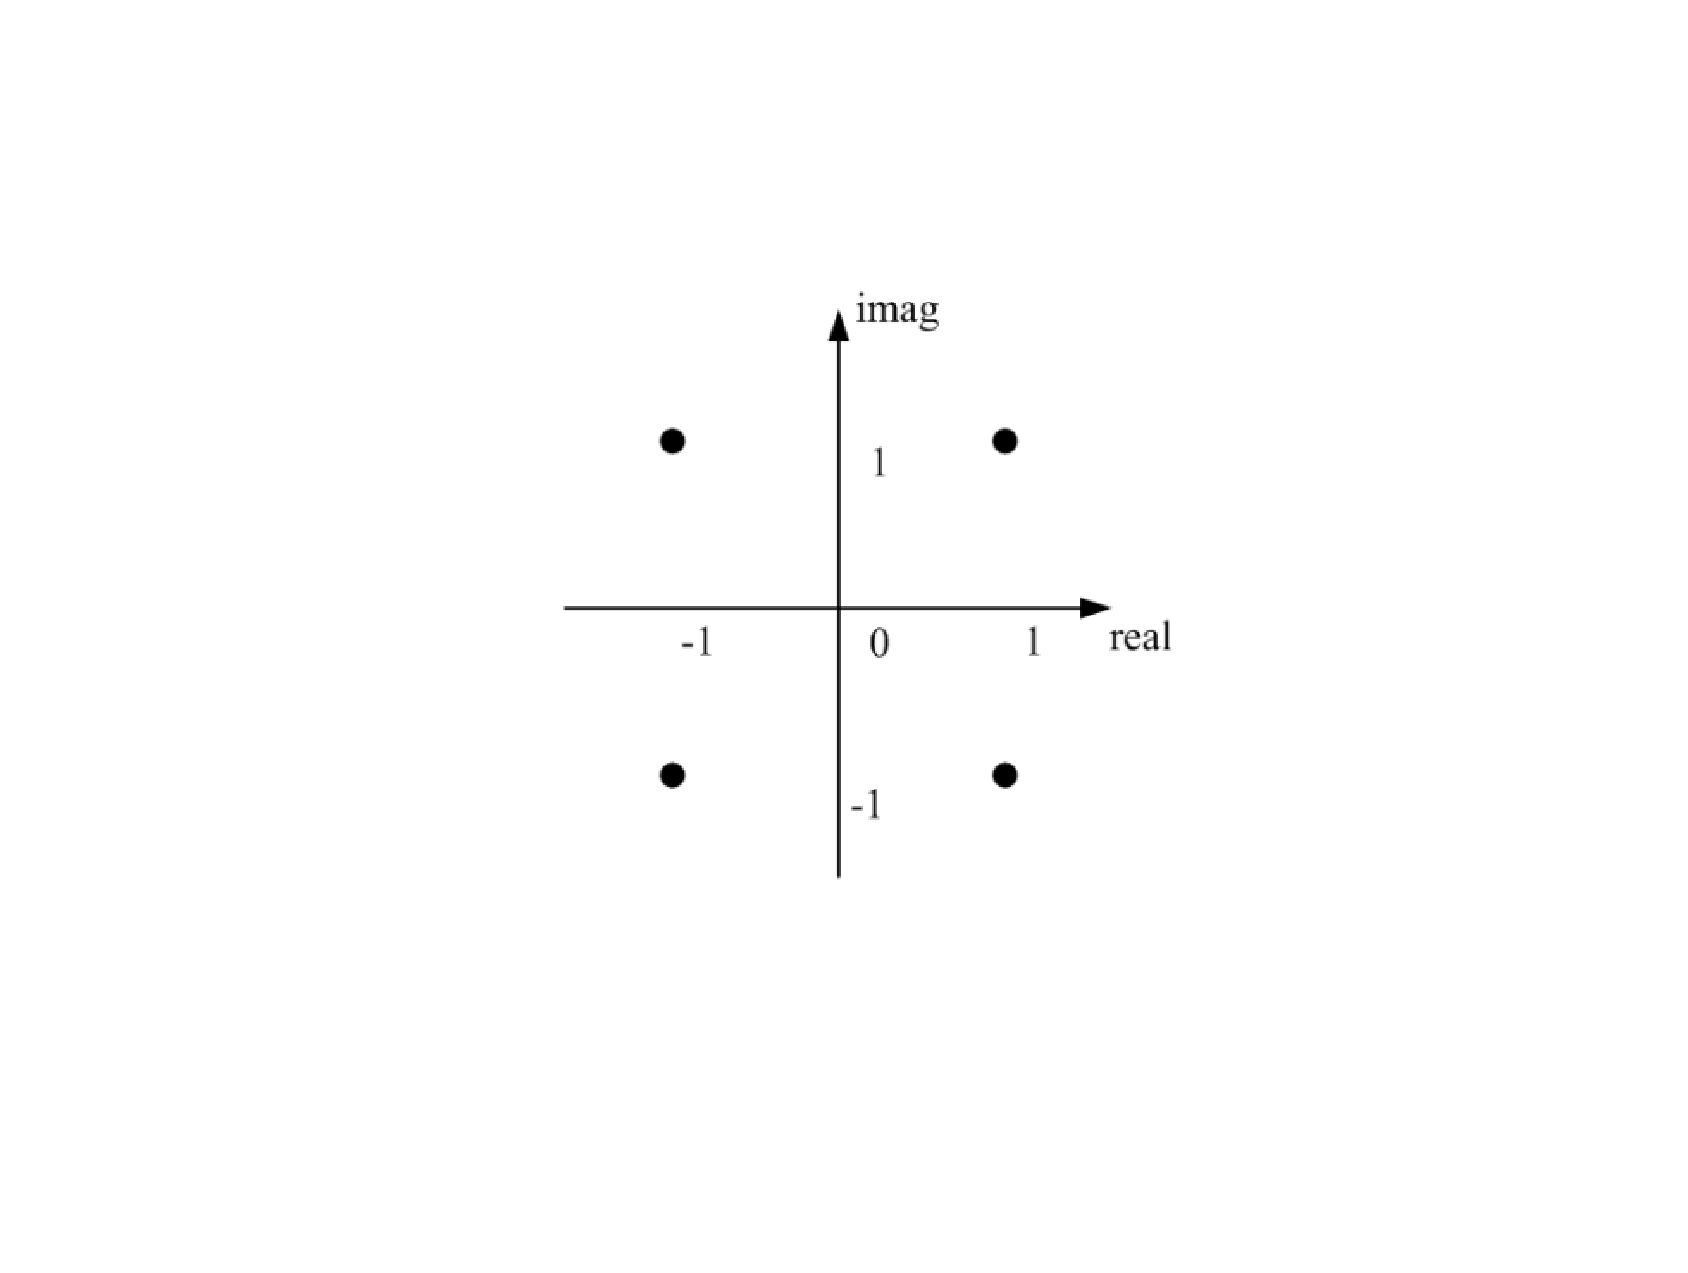
\includegraphics [width=1\columnwidth]{chap2_fig/NOMA_fig2.eps}  %ZICRSystemModel.eps} % {LAR.eps}\columnwidth   [width=2\columnwidth] 
\vspace{-1.5in}
\caption{A complex valued codeword constellation with 4 elements in MUSA. \cite{yuan2016multi}}
\label{fig:noma_fig2}
\end{figure}

An alternative for CDM-NOMA is Multi User Shared Access (MUSA), which was  in \cite{dai2015non}, \cite{yuan2016multi}. In MUSA, short length complex-valued codewords are used to spread user signals before transmission  \cite{yuan2016multi}. The complex valued codewords are constructed from complex valued constellations, with each codeword element picked from the constellation (Fig. \ref{fig:noma_fig2}). User overloading is thus accomplished by increasing the length of the codeword. For a codeword with length of $K$, there will be $4^K$ codewords available thus enabling scalability \cite{yuan2016non}. At the receiver, codeword-level SIC is employed to differentiate user messages. Although MUSA is more scalable then LDS and SCMA, the message recovery process in MUSA introduces the risk of error propagation due to SIC at the receiver. A summary of the discussed NOMA approaches is presented in Table \ref{table:noma}.

\begin{table}[]
\centering
\caption{Summary of discussed NOMA approaches}
\label{table:noma} \scalebox{0.9}{
\begin{tabular}{ccc}
\hline
\textbf{References}					& \textbf{Description}		 			& \textbf{Spectral Efficiency Metric(s)} \\ \hline \hline
\cite{saito2013non} 				& Basic NOMA SIC for PDM-NOMA   & Throughput                             \\ 
\cite{higuchi2013non}       & Beamforming SIC for PDM-NOMA  & Throughput                  \\ 
\cite{hoshyar2008novel}			& LDS for CDM-NOMA							& BER                                    \\
\cite{nikopour2013sparse}		& SCMA for CDM-NOMA							& BER                                    \\
\cite{yuan2016multi}				& MUSA for CDM-NOMA							& BER                                    \\ \hline
\end{tabular}}
\end{table}

%Non-Orthogonal Multiple Access (NOMA), on the other hand, is an alternative technique that can be adopted for spectral efficiency improvements in aeronautical communications. NOMA has been proposed as a next-generation multiple access candidate \cite{dai2015non} in 5G cellular communications. As spectral efficiency is a vital issue that must be addressed in 5G, NOMA, when compared to OMA methods, offers spectral efficiency boosts whilst allowing massive connectivity \cite{dai2015non}.
%
%NOMA allows multiple users to simultaneously share the same spectral resources by allowing an acceptable amount of interference from users simultaneously multiplexed to the same set of spectral resources \cite{dai2015non}. To enable resource multiplexing, NOMA techniques can be broadly categorized as Power Domain Multiplexing (PDM) or Code Domain Multiplexing (CDM).
%
%The NOMA paradigm can be well suited for adaptation for aeronautical communications. PDM-NOMA for instance, can take advantage of the fact that aircrafts on a flight path can be separated by vast distances (e.g. 10km and above). When path loss is considered, interfering signals from nearby aircrafts or ground stations is diminished. Thus, PDM-NOMA can be adopted for both A/G and A/A communications scenarios. CDM-NOMA can also be adopted for aeronautical communications, particularly in congested airspace where a large number of aircrafts are transmitting data via A/G or A/A communication links. In such a scenario, spectral efficiency is improved through simultaneous transmissions achieved via Multi User Shared Access (MUSA) \cite{dai2015non}, \cite{yuan2016multi} or even Sparse Code Multiple Access (SCMA) \cite{nikopour2013sparse}. Interference with legacy aeronautical communications can also be managed if PDM-NOMA or CDM-NOMA techniques are used in combination with D2D/CR related approaches.

\subsubsection{Open Research Problems for Modulation and Multiplexing Schemes in Aeronautical Communications}

The spectral efficiency of ACSs can be improved through suitable modulation schemes. With the current VDL-2 scheme providing low data rates for A/G links, modulation techniques that can transmit more bits per symbol effectively, with simple transceiver designs, can be further investigated. BICM can also be further explored for aeronautical communications usage. In particular, performance analysis of BICM over multipath channels are limited \cite{zhan2017differential}, particularly for combinations of Rician and Rayleigh fading which are expected in aeronautical communications, and can be studied in future works. For SSD, code designs that are suitable for aeronautical communications and the impact of imperfect channel knowledge, particularly for various flight scenarios where Rician fading channels are expected, are also open research problems that must be addressed.

NOMA approaches can also go a long way towards improving the spectral efficiency of ACSs. Although concepts such as frequency reuse, have been applied for aeronautical communications e.g. VDL-2 systems \cite{ribeiro2014framework}, there is further scope to study the feasibility of new NOMA methods for aeronautical communications. By enabling simultaneous sharing of the same frequency band, NOMA provides the capability to support simultaneous transmissions from multiple users in the same channel. When applied to ACSs, NOMA can effectively help to address the scarcity of aeronautical spectrum for communications. 

However, the major downside to such an approach is the inevitable introduction of interference to all NOMA users. In the aeronautical context, this translates to interfering with A/G or even A/A communications. In the worst case, the transmissions of legacy systems in the same band e.g. VHF or L-band, can also be affected. In this aspect, much work will have to be done in the aeronautical context to quantify potential levels of interference to other aircrafts and legacy systems. This is on top of improving PDM-NOMA or CDM-NOMA techniques to reduce delays, error propagation and complexity, which are still open research problems. Finally, future work can also for instance, study the feasibility of incorporating frequency reuse into PDM-NOMA for aeronautical communications.

\subsection{In-Band Full-Duplex Radio Systems for Aeronautical Communications}

% Disscuss relevance to aeronautical communications
The emerging field of In-Band Full-Duplex (IBFD) radio systems can be a direct solution to improve the spectral crunch faced by the aviation community. From the aeronautical communications perspective, IBFD systems enable ACSs, e.g., VDL-2, AeroMACS, LDACS-1 or LDACS-2, the capability to simultaneously transmit and receive signals on the same channel. Therefore, ACSs operating in FD mode can achieve up to twice the spectral efficiency compared to operating in HD mode. Furthermore with proper signal processing techniques, interference and congestion on the aeronautical spectrum between legacy, existing and FD-enabled ACSs can be managed. However, many technical challenges related to interference cancellation/management must be tackled before any aeronautical IBFD communications system can be made feasible.

\subsubsection{SI Cancellation Architectures and the Associated Considerations in Aeronautical Communications}
% Discuss SI technical hurdle and related SI cancellation literature in FD systems
\begin{figure} []
\centering
\vspace{-0.7in}
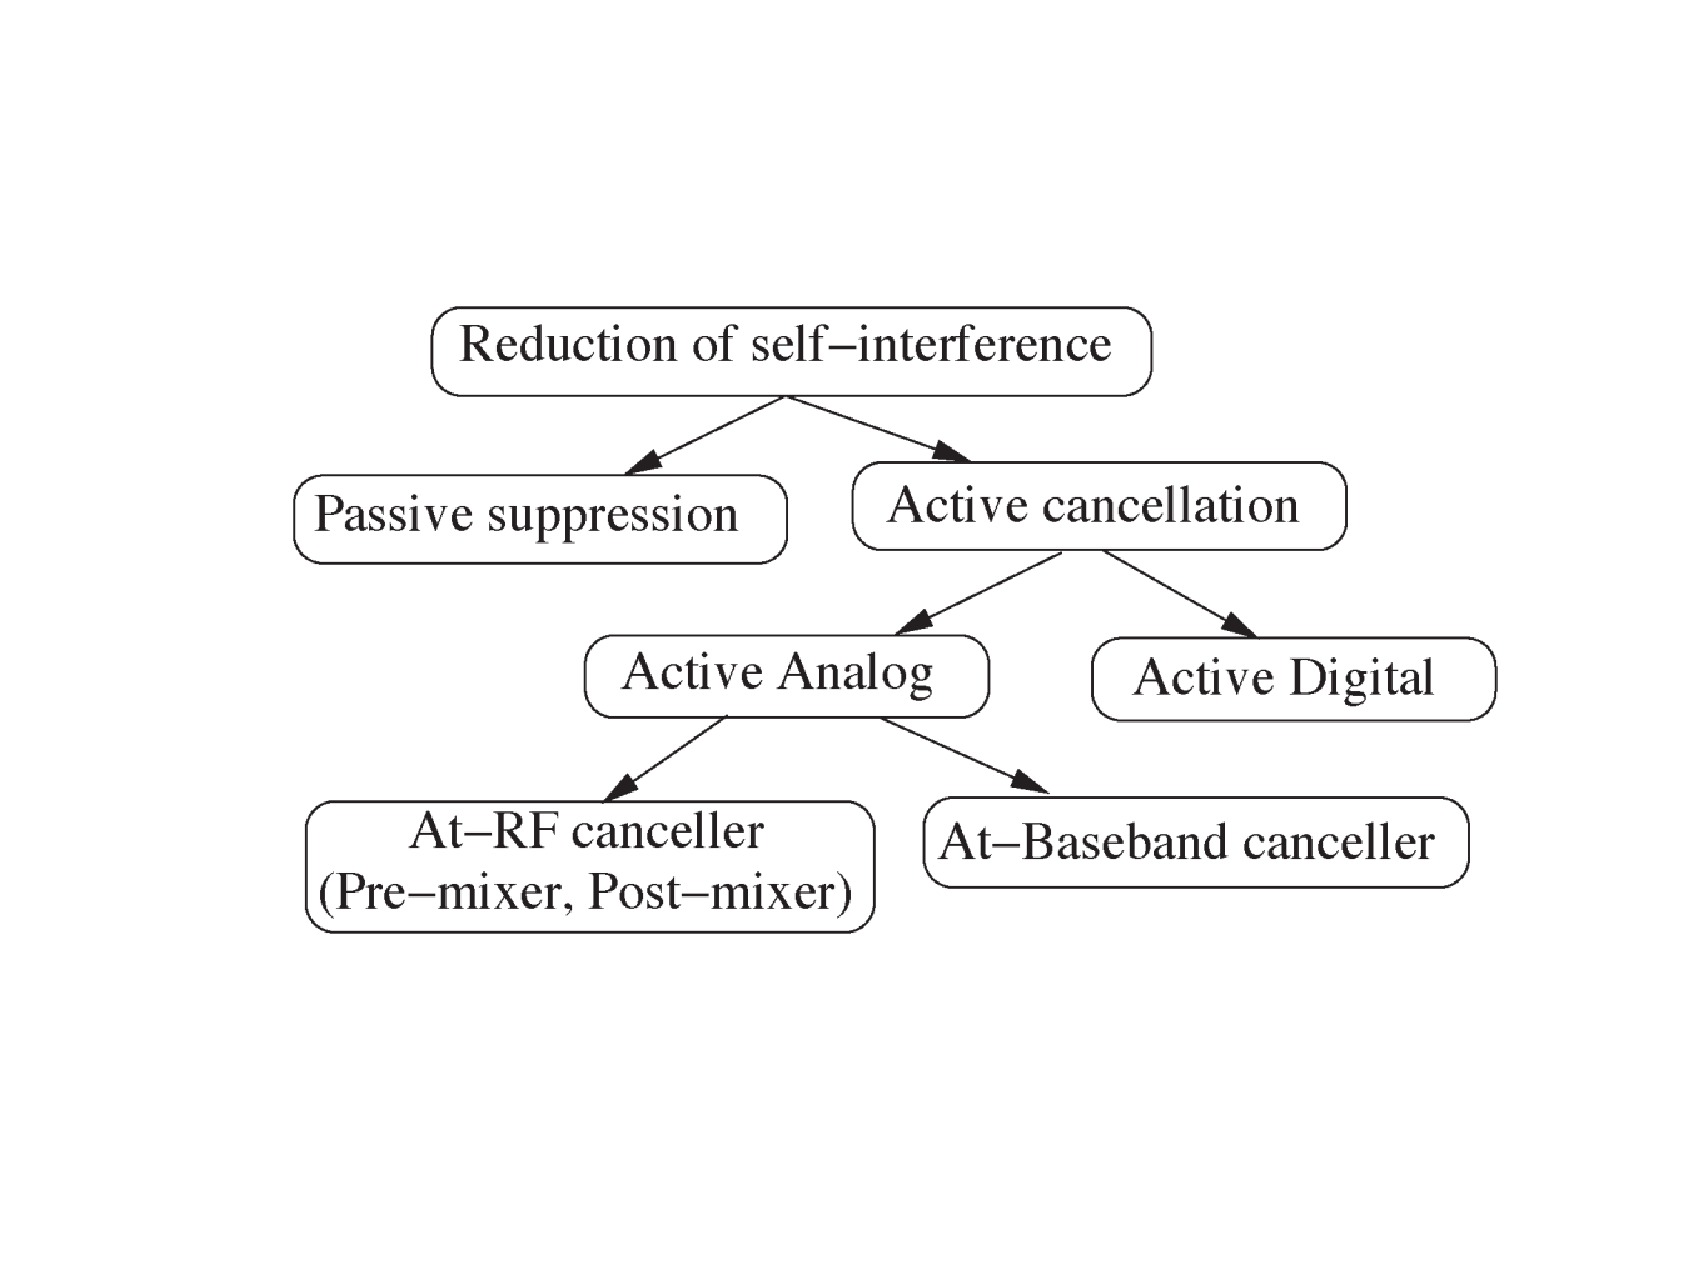
\includegraphics [width=0.7\columnwidth]{chap2_fig/IBFD_fig2.eps} 
\vspace{-0.8in}
\caption{Overview of SI mitigation architectures. \cite{sahai2013impact}.}
\label{fig:IBFD_2}
\end{figure}

One of the major technical hurdles in IBFD systems is the inherent introduction of self interference (SI). A practical IBFD system requires a sufficient level of SI mitigation before communications can become feasible. In this aspect, SI mitigation architectures can be categorized into either passive suppression or active cancellation \cite{sahai2013impact} (Fig. \ref{fig:IBFD_2}). The former entails SI mitigation via antenna separation (separate antenna IBFD systems) \cite{duarte2014design,ahmed2012simultaneous} or circulator isolation (shared antenna IBFD systems) \cite{bharadia2013full,huberman2015mimo} while the latter cancels SI either in the analog or digital domain. 

Active analog/digital SI cancellation architectures are further categorized as pre-mixer, post-mixer or baseband cancelers. A mixture of pre, post and baseband cancelers in the same architecture is also possible. In a pre-mixer canceler, the processing of the cancellation signal is performed before the RF mixer, e.g., having a parallel radio chain \cite{ahmed2015all}. Likewise, a post-mixer canceler processes the cancellation signal after the RF mixer, e.g., Balun (Balance/Unbalance) cancellation \cite{jain2011practical} while a baseband canceler processes the canceling signal at the baseband level.

% Discuss open problems related to SI mitigation
It should be noted that digital and analog SI cancellation both experience unique limitations \cite{sahai2013impact}. In digital SI cancellation, the strength of the resultant SI signal before it enters the ADC is high. Consequently, SI mitigation becomes ineffective since the SI signal will still be above the receiver noise floor after digital SI cancellation due to limited ADC dynamic range \cite{sabharwal2014band}. In analog SI cancellation, SI mitigation will require complex hardware \cite{everett2016softnull}, thus potentially increasing the physical size of transceivers and contributing to overall size, weight and power requirements for FD-enabled avionics. 

On top of the associated limitations for both digital and analog SI cancellation, residual SI will also be present in the form of phase noise. The residual SI is a result of imperfect SI channel estimation at the FD transceiver \cite{sahai2013impact} and it can be the limiting factor in practical IBFD systems. In addition, suitable SI mitigation architectures of IBFD systems (e.g. active or passive) will need to be investigated to determine a suitable architecture for aeronautical usage, on top of accurate theoretical modeling of SI signals and multipath fading effects in an aeronautical channel e.g. Rician or Rayleigh fading environments \cite{haas2002aeronautical}.

\subsubsection{Hybrid-Duplex Systems for Aeronautical Communications}
% Discuss HBD systems as a way to transition towards a newer generation of FD-enabled ACSs
Apart from suitable SI mitigation architectures and the associated considerations for aeronautical communications, transiting towards a new generation of FD-enabled ACSs is likely to be disruptive as legacy HD ACSs must first be replaced. To ease the transition from legacy HD to a FD-enabled ACS, a hybrid-duplex (HBD) ACS consisting of HD and FD aircrafts/ground stations, e.g., Fig. \ref{fig:chap2_fd_gs_system_model}, is a viable alternative. 

Already, HBD systems have been seen in cognitive radio systems \cite{li2014linear} and cellular systems \cite{yin2013full,jang2015spatial,cirik2016robust} where nodes operating in either HD or FD have been studied. The main obstacle in such a HBD system is the inherent SI as a result of simultaneous signal transmission and reception. As a result, sufficient levels of SI mitigation must be achieved to enable the co-existence of multiple ACSs operating on the same frequency. In this aspect, concepts related to NOMA can be adapted for FD operations. Future studies can look at the suitability of incorporating Successive Interference Cancellation (SIC) from power-domain NOMA \cite{yan2015receiver}, \cite{huang2016full}, \cite{ali2016dynamic}, \cite{zhang2016full} into multi-user IBFD wireless systems. Other studies can also look at using code-domain NOMA concepts such as MUSA or SCMA \cite{yuan2016multi}, \cite{nikopour2013sparse}. 

Apart from SI, HBD systems must also manage interference from nearby HD nodes, e.g., HD avionics, as seen in Fig. \ref{fig:chap2_fd_gs_system_model}a. Interference management strategies have long been an area of active research in the literature, particularly from the information theoretic perspective. For instance, studies investigating interference management approaches that do not consider any inherent structure in the interference, such as interference avoidance, have been noted \cite{qu2014understanding}. Such interference avoidance strategies, which are typically based on either random access, e.g., contention-based channel access, or deterministic access, e.g., orthogonal multiple access, hinders spectral efficiency \cite{qu2014understanding,weber2007transmission}. Therefore, exploiting the structure of interference, i.e., interference management, has been the topic of keen research interest in recent years \cite{qu2014understanding} to achieve better performance \cite{weber2007transmission} and spectral efficiency in multi-user systems. 

In aeronautical communications, the distances between aircrafts affects the level of interference experienced at the HD avionics. Long separation distances between aircrafts results in weak interference scenarios and vice-versa. Accordingly, suitable interference management techniques must be employed for different interference scenarios. For weak interference scenarios, it has been known that the optimal interference management strategy is to treat interference as noise, i.e., interference ignorant (II) \cite{annapureddy2009gaussian,zahavi2017cooperation} detector. In contrast, decoding and then removing interference from the received signal, i.e, successive interference cancellation (SIC) detector, is an effective interference management strategy in strong interference scenarios \cite{qu2014understanding,weber2007transmission}. The joint detection (JD) strategy is also another effective interference management strategy when the interfering signal is sufficiently strong \cite{zahavi2017cooperation,zhou2015mac,shubhi2017joint,blomer2009transmission}. In particular, the joint detector is optimal from the sum-rate perspective, when interference is sufficiently strong, for an additive white Gaussian noise channel \cite{zahavi2017cooperation} at the cost of computational complexity \cite{zhou2015mac,shubhi2017joint}.

To measure the effectiveness of the various interference management strategies in HBD systems, outage probability can be analyzed. In the literature, outage probability for many statistical distributions has been extensively studied. For the II detector, outage probability for Gamma distributed signals \cite{yao1992investigations}, composite fading consisting of exponentially distributed signal-of-interest (SOI) and squared ${\mathcal{K}}$-distributed interfering signals \cite{bithas2015mobile}, and non-centered Chi-squared distributed signals \cite{rached2017unified} are available in closed-form. 

For the SIC detector, closed-form outage probability expressions for combinations of non-centered Chi-squared, exponential or Gamma distributed SOI with exponentially distributed interfering signals were studied in \cite{hasna2003performance,romero2008receive}. However, both \cite{hasna2003performance} and \cite{romero2008receive} assumed partial SIC where at least one interferer remain after interference cancellation and thus, performance analysis involving full SIC cannot be obtained. The outage probability of full SIC with exponentially distributed signals was analyzed in \cite{zhang2017full} and to the best of our knowledge, similar outage analysis for non-centered Chi-squared distribution is not yet available in the literature. Finally, for the joint detector, outage analysis is only available for exponentially distributed signals, as presented in \cite{narasimhan2007individual}, and similar studies involving non-centered Chi-squared distribution are unavailable in the literature.

Finite SNR diversity gain and finite SNR diversity-multiplexing trade-off (DMT) are also metrics that can measure the effectiveness of the various interference management strategies in HBD systems. For fixed transmission rate systems, reliability is quantified through finite SNR diversity gain by computing the outage probability decay rate at a fixed SNR \cite{shin2008diversity}. Reliability in variable transmission rate systems is similarly quantified through finite SNR DMT, with the transmission rate, i.e., multiplexing gain, taken into consideration \cite{narasimhan2006finite}. 

Although diversity gains have long been analyzed at asymptotic SNRs, a gradual shift in research interest towards the low-to-moderate SNR regime has been seen due to the practical relevance in the evaluation of system performance. In particular, wireless systems typically operate at low-to-moderate SNR regimes, and through finite SNR analysis, changes in outage probability behavior can be observed \cite{shin2008diversity}. Knowing a system's outage probability behavior at low-to-moderate SNR regimes is essential in providing accurate system performance analysis as it reveals the SNR needed before a particular level of reliability, i.e., Quality-of-Service (QoS), is attainable through effective code designs, e.g., turbo codes, low-density parity-check codes and space-time codes \cite{narasimhan2006finite}. Finite SNR analysis also allows the identification of the multiplexing gain region (MGR) \cite{karmakar2012generalized}. The MGR indicates the range of multiplexing gains for which non-zero diversity gains is attainable in a multi-user channel. In aeronautical communications, MGRs enable system designers to determine the QoS requirements of ACSs and extensive analysis on this topic is unavailable in the literature.

\subsubsection{Integration of In-Band Full-Duplex Cognitive Radio Systems for Aeronautical Communications}

One of the key reasons behind the shortage of available spectrum for aeronautical communications stems from the inefficient allocation of radio channels \cite{jacob2016cognitive}. In particular, radio channels used in aeronautical communications are often assigned to specific geographical areas \cite{jacob2016cognitive} or ACSs \cite{jamal2017fbmc}, e.g., distance measuring equipment (DME), on a permanent basis. The static allocation of the aeronautical spectrum exasperates the issue of spectral efficiency due to inefficient utilization of spectral resources, where spectrum utilization as low as 5\% has been reported \cite{jacob2016cognitive}. In the L-band, the static allocation of the aeronautical spectrum has resulted in unused spectrum, i.e., white space, between adjacent DMEs \cite{jamal2017fbmc}. Although LDACS-1 and LDACS-2 can be deployed to operate within the white space \cite{schnell2014ldacs,jamal2017fbmc}, spectral efficiency can be further improved through the introduction of FD-enabled cognitive radio (CR) systems in aeronautical communications.  

% elaborate more on what kind of channel models we can use, whether the SU or PU operates in FD, which node (GS or AS?) utilizes CR.
Unlike in HD CR systems, FD-enabled CR systems have the capability to simultaneously transmit signals while sensing the spectrum \cite{amjad2017full}. CR applications in the context of aeronautical communications have been studied in the literature for A/G \cite{wang2010cognitive,zhang2015aeronautical} and unmanned aerial vehicle (UAV) communications \cite{saleem2015integration,chen2011collaborative}, with ground stations (GSs) and air-stations (ASs) alike playing the role of either primary users (PUs) or secondary users (SUs).

The utilization of the white space also differs from HD CR systems. In the underlay mode of operation, the transmissions of the SUs and PUs in HD CR systems are controlled such that the interference experienced by the PUs is sufficiently low \cite{amjad2017full}. The underlay mode of operation in FD-enabled CR systems is similar except that both PUs and SUs transmit on the same spectrum \cite{amjad2017full,gaafar2017underlay}. For the overlay mode of operation, SUs in HD CR systems vary transmission characteristics to avoid interfering with PUs on the same frequency band \cite{amjad2017full}. However, in FD-enabled CR systems, PUs and SUs simultaneously transmit on the same frequency and SUs vary transmission characteristics to reduce SI \cite{amjad2017full,amin2017overlay}. In the interweave mode of operation, SUs only operate when the PUs are not transmitting for both HD and FD-enabled CR systems \cite{amjad2017full,liao2014listen}. The only difference between HD and FD-enabled CR systems in interweave mode is that SUs in the latter simultaneously sense and transmit signals, thus improving spectrum utilization. Finally, hybrid modes of operation are also possible in FD-enabled CR systems, e.g., in \cite{afifi2015incorporating} where SUs either sense-and-transmit or transmit-and-receive signals simultaneously.

The nature of FD-enabled CR systems enables the activities of the PUs and the SUs to be monitored much more effectively than HD CR systems. As such, interference management strategies used in HBD systems can be readily adopted to manage the interference between PUs and SUs. For instance, the II approach to interference management can be adopted for use in FD-enabled CR systems operating in underlay mode. Interference management strategies based on SIC and JD approaches can also be employed for FD-enabled CR systems operating in overlay mode. The performance analysis done for HBD systems, e.g., outage probability and finite SNR diversity gain, can also be applied in FD-enabled CR systems to gauge performance at both node and system level.

\subsubsection{Open Research Problems of In-Band Full-Duplex Systems for Aeronautical Communications}

% Discuss the potential open problems of FD-enabled ACS
Employing the in-band full-duplex paradigm to address spectral efficiency in aeronautical communications is a very attractive solution. As seen in this section, spectrum utilization can be twice as effective in FD-enabled systems than HD systems. From the aeronautical communications perspective, realistic performance analysis of FD-enabled ACSs must take into consideration scenarios involving an aircraft that is en route, landing, taking-off or parking. In addition, the impact of inter-aircraft interference and residual SI must be examined in detail, before a fair assessment of FD-enabled ACSs is made possible. To this end, outage probability and finite SNR diversity gain are effective metrics that can provide system designers with theoretical node and system level performance. These metrics can be adopted for both HBD systems and FD-enabled CR systems in aeronautical communications.

Outage probability computations for FD-enabled ACSs must involve aircrafts and GS communicating in en route, landing, taking-off or parking scenarios, where fading is encountered. Since inter-aircraft interference and SI are also present, outage probability expressions in an interference-limited environment consisting of either Rician fading, Rayleigh fading, or combinations of both, must be derived for interference management strategies based on II, SIC or JD. For Rician fading environments, closed-form outage probability expressions are only available in \cite{rached2017unified} for the II-based interference management strategy. For both SIC and JD interference management strategies in Rician fading environments, closed-form outage probability expressions are not available in the literature. 

In \cite{rached2017unified}, the authors proposed an innovative moment-based approach to evaluate outage probability by expressing the probability density functions (PDFs) of the SOI and the interfering signal into the power series equivalent for various statistical distributions. The same approach can also be extended to evaluate both the SIC and JD interference management approaches to potentially yield closed-form outage probability expressions, along with provisions of the necessary convergence tests. The resultant outage analysis can be used to determine the impact of residual SI and inter-aircraft interference at both node and system level and compared against HD ACSs. For various inter-aircraft interference levels, suitable interference management strategies can also be identified.

The closed-form outage probability expressions, in the form of power series, for the II, SIC and JD approaches can be used as platforms to derive closed-form finite SNR diversity gain expressions. In particular, the finite SNR diversity gains of fixed and variable rate ACSs can be quantified and analyzed in detail to determine reliability, i.e., QoS, under various inter-aircraft interference levels. From the derived closed-form finite SNR diversity gain expressions, the MGR of the II, SIC and JD approaches be plotted to reveal the respective range of supported QoS requirements for A/G and A/A communications.

The resultant conclusions from both outage and finite SNR diversity gain analysis can then be used to identify A/G or A/A communication scenarios in which FD-based ACSs either performs the same as, or outperforms HD-based ACSs. Furthermore, outage and finite SNR diversity gain analysis can be used to determine the upper and lower bound of BER performance for both FD-based and HD-based ACSs. Future studies can also look at simulating various modulation techniques such as BPSK, QPSK, 8-PSK, D8PSK and QAM to determine if any of these modulation techniques are well suited for FD operations. The incorporation of constellation rotation and its effects on BER performance can also be studied for both FD-based and HD-based ACSs. These studies can also identify the ideal operating scenarios for practical systems, e.g., identifying ideal scenarios for constellation rotation in ACSs.

\section{Summary}
With growing air traffic projected in the near future, the issue of spectral efficiency in aeronautical communications will be a critical problem that must be addressed in due time by the aviation industry. In this chapter, works pertaining to the state-of-the-art in aeronautical communications was surveyed, with AeroMACS, satellite communications and LDACS earmarked as candidate technologies for airport, remote and continental communications respectively. Techniques ranging from CR and D2D communications to NOMA and IBFD radio was also surveyed as potential methods to improve spectral efficiency in aeronautical communications. Finally, the possible adaptation of earlier highlighted spectral efficiency approaches to further improve spectral efficiency in the aeronautical context was presented as possible research opportunities in aeronautical communications. The feasibility of employing general spectral efficiency improvement techniques such as IBFD radio systems and NOMA was also discussed, with potential open research problems highlighted.




